\section{Wasserfallmodell}

\begin{tcolorbox}[title=Wasserfallmodell]
    Das \textbf{Wasserfallmodell} ist ein \textbf{sequentielles} und \textbf{dokumentengetriebenes} Phasenmodell und in \textbf{6 Phasen} aufgeteilt. Die Ergebnisse der Phasen sind \textit{Dokumente},\textit{Modelle},\textit{Code} oder \textit{Testprotokolle}, die man zusammenfassen als \textbf{Artefakte} bezeichnet.
    \begin{itemize}
        \item Die Phasen des Wasserfallmodells folgen \textbf{strikt hintereinander}.
        \item Ergebnisse abgeschlossener Phasen werden nicht mehr geändert.
        \item Stellt sich heraus, dass in einer vorhergehenden Phase schwerwiegende Fehler begangen wurden, muss das gesamte Team in diese Phase zurückspringen, den Fehler beheben und von da an jede nachfolgende Phase erneut durchlaufen.
        \item[] $\rightarrow$ Voraussetzung für ein erfolgreiches Arbeiten mit diesem Modell ist eine vollständige und fehlerfreie Erstellung von Artefakten in jeder Phase
        \item \textbf{Vorteile}:
        \begin{itemize}
            \item Bei überschaubaren Projekten bietet das Modell eine genauere Planbarkeit, da spätestens nach dem Entwurf klar ist, welche Arbeiten erledigt werden müssen.
            \item Die initiale Planung ist in drei Phasen eingeteilt (Anforderung, Analyse, Entwurf), in denen die zu erledigenden Tätigkeiten herausgearbeitet werden können.
        \end{itemize}
        \item \textbf{Nachteile}: Bei kaum überschaubaren Objekten bzw. in Projekten mit hoher Eigendynamik und sich laufend ändernden Anforderungen ist das Projekt zu rigide und erlaubt keine angemessene Flexibilität.
    \end{itemize}
\end{tcolorbox}

\begin{table}[]
    \centering
    \setlength{\tabcolsep}{0.5em}
    \def\arraystretch{1.5}
    \begin{tabular}{|c|l|}
        \hline
        \textbf{Phase} & \textbf{Ergebnis}                                             \\ \hline
         1. Anforderungsphase      & Lastenheft, Pflichtenheft\\ \hline
        2. Analysephase      & DV-Konzept, Domänenmodell \\ \hline
        3. Entwurfsphase      & Fachkonzept, UML-Modelle, Architektur \\ \hline
        4. Implementierungsphase      & Quellcode, Datenbankschemen, Tests \\ \hline
        5. Integrations- \& Testphase      & Testfälle, Testprotokolle \\ \hline
        6. Einführung und Wartung      & - \\ \hline
    \end{tabular}
    \caption{Phasen und Ergebnisse des Wasserfallmodells}
\end{table}



\begin{figure}
    \centering
    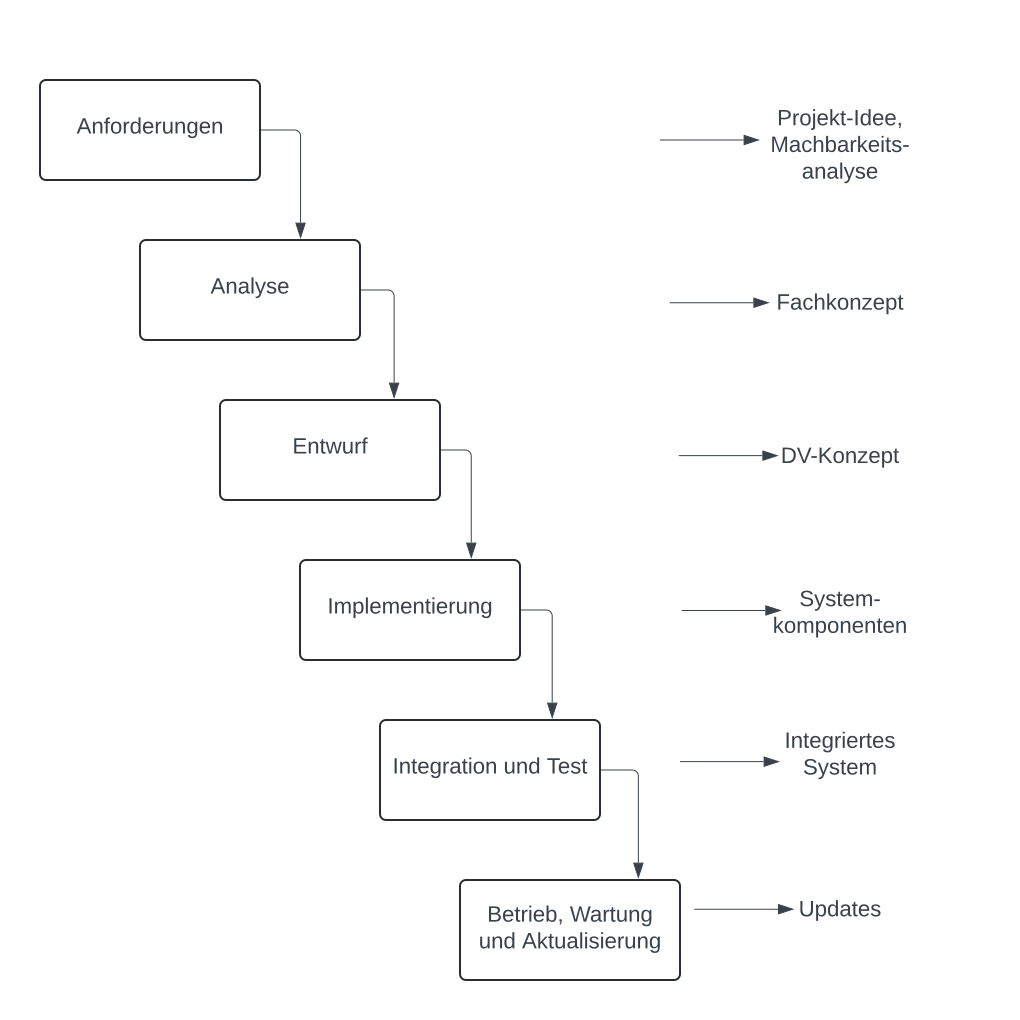
\includegraphics[scale=0.3]{chapters/Anhang/CheatSheets/img/wasserfallmodell}
    \caption{Phasen des Wasserfallmodells. (Quelle: in Anlehnung an \cite[318, Abbildung 14-3]{AABG14n})}
    \label{fig:wasserfallmodell_cc}
\end{figure}